\documentclass{article}
\linespread{0.7}
\usepackage[a4paper, margin=3mm, landscape]{geometry}
\usepackage{multicol}
\usepackage{xcolor}
\usepackage{enumitem}
\usepackage{amsmath}
\usepackage{amsfonts}
\usepackage{listings}
\usepackage{soul}
\usepackage{graphicx}

\pdfinfo{
    /Title (ACC1701x.pdf)
    /Creator (TeX)
    /Producer (pdfTeX 1.40.0)
    /Author (Vincent Pang)
    /Subject (ACC1701x)
    /Keywords (ACC1701x, nus, cheatsheet, pdf)
}

\graphicspath{ {./img/} }

\pagestyle{empty}
\setcounter{secnumdepth}{0}
\setlength{\columnseprule}{0.25pt}

% Redefine section commands to use less space
\makeatletter
\renewcommand{\section}{\@startsection{section}{1}{0mm}%
    {-1ex plus -.5ex minus -.2ex}%
    {0.5ex plus .2ex}%x
{\normalfont\large\bfseries}}
\renewcommand{\subsection}{\@startsection{subsection}{2}{0mm}%
    {-1explus -.5ex minus -.2ex}%
    {0.5ex plus .2ex}%
{\normalfont\normalsize\bfseries}}
\renewcommand{\subsubsection}{\@startsection{subsubsection}{3}{0mm}%
    {-1ex plus -.5ex minus -.2ex}%
    {1ex plus .2ex}%
{\normalfont\small\bfseries}}%
\makeatother

% Adjust spacing for all itemize/enumerate
\setlength{\leftmargini}{0.5cm}
\setlength{\leftmarginii}{0.5cm}
\setlist[itemize,1]{leftmargin=2mm,labelindent=1mm,labelsep=1mm}
\setlist[itemize,2]{leftmargin=2mm,labelindent=1mm,labelsep=1mm}

% Font
\renewcommand{\familydefault}{\sfdefault}

% Define colors for math formulas
\definecolor{myblue}{cmyk}{1,.72,0,.38}
\everymath\expandafter{\the\everymath \color{myblue}}

% Custom command for keywords
\definecolor{highlight}{RGB}{251,243,218}
\newcommand{\keyword}[2][]{\sethlcolor{highlight}\hl{\textbf{#2}} #1 - }
\newcommand{\ilkeyword}[1]{\sethlcolor{highlight}\hl{\textbf{#1}}}

% Define colors and style for code
\definecolor{codegreen}{rgb}{0,0.6,0}
\definecolor{codegray}{rgb}{0.5,0.5,0.5}
\definecolor{codered}{HTML}{CC241D}
\definecolor{backcolor}{rgb}{0.95,0.95,0.95}
\lstdefinestyle{codestyle}{
    backgroundcolor = \color{backcolor},
    commentstyle = \color{codegray},
    keywordstyle = \color{codered},
    stringstyle = \color{codegreen},
    basicstyle = \ttfamily,
    breakatwhitespace = false,
    showstringspaces = false,
    breaklines = true,
    showtabs = false,
    tabsize = 2
}
\lstset{style = codestyle}

% -----------------------------------------------------------------------
\begin{document}
\begin{multicols*}{3}
\small
\footnotesize

% Title box
\begin{center}
    \fbox{
        \parbox{0.8\linewidth}{
            \centering \textcolor{black}{
                {\Large\textbf{ACC1701x}} \\
                \normalsize{AY22/23 Sem 2}} \\
                {\footnotesize \textcolor{gray}{github.com/securespider}}
        }
    }
\end{center}
%-----------------------------------------------------------------------------------------------------------------------
\section{01. Financial Statements}
\keyword{Consolidated Financial Statements}{Financial information about the group of companies including parent and subsidiaries}
\\How does a parent company control subsidiary?
\begin{itemize}
	\item Own a controlling interest of subsidiary's share
	\item Remaining shares are \keyword{Non controlling interest}{Separated, under book value}
\end{itemize}
\keyword{Associate Companies}{Interest in shares outside group that wields significant influence}
\begin{itemize}
	\item Includes one-line partial consolidation of associate company in book value
	\item Recorded using equity method
\end{itemize}

\subsection{Consolidated Balance Sheet}
Purpose
\begin{itemize}
	\item Report net worth of group \textbf{at specific date}
\end{itemize}
\subsubsection{Fundamental Accounting Equation} 
\begin{description}
	\item \textit{Assets = Liabilities + Equity}
	\item[Assets]{Resource controlled by company (eg. cash, accounts receivable, inventory, land, equipment, buildings)}
	\item[Liabilities]{Amount owed to others leading to outflow of resources (eg. accounts payable, expenses)}
	\item[Equity]{Owner's claim on residual interest after deducting liabilities}
\end{description}
\subsubsection{Problems}
\begin{enumerate}
	\item Not market value
	\begin{itemize}
		\item Does not tell what the equity is worth in market
		\item Market value = market share price * outstanding shares
	\end{itemize}
	\item Mixed measurement model - Mathematically dubious calculation 
	\begin{itemize}
		\item Property measured using \keyword{cost less depreciation}{amount originally paid less depreciation}, OR current market value
	\end{itemize}
\end{enumerate}
\subsubsection{Motivation}
\begin{enumerate}
	\item Comparing
	\begin{itemize}
		\item Compare companies using \keyword{Market-to-book ratio}{$\dfrac{Market~value}{Total~equity}$}
		\item Why are they not the same?
		\begin{itemize}
			\item Market takes into account future prospects not captured by book value
		\end{itemize}
	\end{itemize}
	
	\item Details
	\begin{itemize}
		\item Provides useful information
	\end{itemize}
\end{enumerate}

\subsection{Statement of Changes in Equity}
Lists impact of events on changes in equity
\subsubsection{Factors}
\begin{enumerate}
	\item Contributions from shareholders
	\item Distributions to shareholders
	\item Business income/expenses
	\item \keyword{Capital maintenance adjustments}{Remeasurement of asset/liability value}
\end{enumerate}

\subsection{Statement of Comprehensive Income}
\begin{itemize}
	\item \keyword{Comprehensive Income}{Reflects changes of equity from non-owner sources and traditional income}
	\item Show all operating and financial events that affect non-owners' interest in business
	\item Includes unrealised gains and losses

\end{itemize}

\subsubsection{Income Statement}
Includes information about business income and expenses for \textbf{the year}

\subsection{Statement of Cash Flows}
\keyword{Accrual Basis}{Record values when exchange of goods and services \textbf{NOT cash flows}}
\subsubsection{Subsections}
\begin{itemize}
	\item Operating activities
	\item Investing activities
	\item \keyword{Financing activities}{Borrowing or issuing shares (eg. repayments, share buybacks)}
\end{itemize}

\subsection{Item Breakdown}
\begin{description}
	\item[Current assets/liabilities]{Likely to be converted to cash/settled within a year}
	\item[PPE]{Property, plant and equipment used in business}
	\item[Right-of-use assets]{Rented premises for business (Asset)}
	\item[Lease liabilities]{Outstanding rental payments wrt ROU assets}
	\item[Trade Receivables]{Outstanding dues from \textbf{credit} customers}
	\item[Cost of Goods Sold(COGS)]{Amount paid to suppliers for goods sold to customers}
	\item[Gross Profit]{= COGS - Sales}
	\item[Interest Income and expense]{Profit from investing and financing activities}
\end{description}
%-----------------------------------------------------------------------------------------------------------------------
\section{02. Ratios}
\begin{itemize}
	\item Comparing companies as investment opportunities
	\item Comparing previous years to measure progress
	\item Overcome difference in scale
\end{itemize}
\subsubsection{Terms}
\begin{description}
	\item[Net Profit]{Profits after tax but before calculating non-controlling interests}
	\item[Net Sales]{Sales after adjusting for discounts and returned goods (Revenue)}
	\item[Profits attributable to ordinary shareholders of the parent company]{Profits excluding non-controlling interest}
	\item[Short-term financial assets]{Fixed deposits, shares that can be converted to cash within a year}
\end{description}

\subsection{Profitability Ratios}
\begin{itemize}
	\item Measures performance of company over the year
\end{itemize}
\begin{description}
	\item[Profit Margin]{$\dfrac{Net~Profits}{Net~sales}$}
	\item[Return on total assets]{$\dfrac{Net~Profit}{Average~Total~Assets}$}
	\item[Return on ordinary shareholders' equity]{$\dfrac{Net~Profit}{Average~total~equity}$}
	\begin{itemize}
		\item Equity should be net of any dividends\slash other equity instruments
	\end{itemize}
	\item[Earnings per share]{$\dfrac{Ordinary~shareholders~profits-Pref~Dividends}{Weighted~average~number~of~shares~during~year}$}
\end{description}
\subsubsection{Equity Categories}
\begin{itemize}
	\item \keyword{Share capital}{Amount collected when company originally issued shares}
	\item \keyword{Retained earnings}{Accumulated profits - Amount paid as dividents}
\end{itemize}

\subsection{Liquidity and efficiency ratios}
\begin{itemize}
	\item Examine company capacity to meet short term debt obligation with current assets
\end{itemize}
\begin{description}
	\item[Current ratio]{$\dfrac{Current~assets}{Current~liabilities}$}
	\item[Acid Test ratio]{$\dfrac{Cash+Short~term~fin~assets+Current~receivables}{Current~liabilities}$}
	\item[Accounts receivable turnover]{$\dfrac{Net~Sales}{Average~accounts~(Trade)~receivables}$}
	\begin{itemize}
		\item Receivables is \keyword{net}{Adjustment made for customers who may default}
	\end{itemize}
	\item[Inventory Turnover]{$\dfrac{Cost~of~goods~sold}{Average~inventory}$}
	\item[Accounts payable turnover]{$\dfrac{Cost~of~goods~sold}{Average~accounts~(trade)~payable}$}
	\item[Days' sales uncollected]{$\dfrac{Accounts~(Trade)~receivables,~net}{Net~sales}*365$}
	\item[Days' sales in inventory]{$\dfrac{Ending~Inventory}{Cost~of~goods~sold}*365$}
	\item[Days' purchases in accounts payable]{$\dfrac{Account~(trade)~payable}{Cost~of~goods~sold}*365$}
	\item[Total Asset Turnover]{$\dfrac{Net~sales}{Average~total~assets}$}
\end{description}

\subsubsection{Prepaid flows}
\begin{itemize}
	\item \keyword{Prepaid Expense}{Payments made for services not yet received (Assets)}
	\item \keyword{Unearned Revenue}{Advanced payments received from customers (Liabilities)}
\end{itemize}

\subsection{Solvency Ratios}
\begin{itemize}
	\item Identify the company's risk of going bankrupt
	\item Gauge company chances of staying afloat
\end{itemize}
\begin{description}
	\item[Debt Ratio]{$\dfrac{Total~liabilities}{Total~assets}$}
	\item[Equity Ratio]{$\dfrac{Total~equity}{Total~assets}$}
	\item[Times interest earned]{$\dfrac{Profit~before~interest~expense/tax}{Interes~expense}$}
	\item[Debt to equity ratio]{$\dfrac{Total~Liabilities}{Total~equity}$}
\end{description}

\subsection{Market prospects ratio}
\begin{itemize}
	\item Help compare share price to other investments
\end{itemize}

\begin{description}
	\item[Price-earnings ratio]{$\dfrac{Market~price~per~ordinary~share}{Earnings~per~share}$}
	\item[Divident yield]{$\dfrac{Annual~cash~dividents~per~share}{Market~price~per~share}$}
\end{description}

%-----------------------------------------------------------------------------------------------------------------------
\section{03. Accounting Equation}
\keyword{Sole Proprietorship}{Business owned by a single party}
$\triangle Capital=Capital~contributed+Income-Expenses+Withdrawals$
\subsection{Concepts}
\begin{itemize}
	\item \keyword{Accrual accounting}{Revenue and expenses recorded when goods and services change hands}
	\item \keyword{Income}{Increase in equity net from any contributions}
	\item \keyword{Expense}{Decrease in equity net from withdrawals}
\end{itemize}
\begin{enumerate}
	\item{Income statement}{Records revenues, expenses and net profit}
	\item{Statements of changes in equity}
	\begin{itemize}
		\item{Records changes in a month}
		\item{Includes contributions from owners and withdrawals}
	\end{itemize}
	\item Balance sheet
	\begin{itemize}
		\item{Refers to a specific date so must specify date}
		\item{Breakdown assets and liabilities}
	\end{itemize}
	\item Statements of cash flow
	\begin{description}
		\item{Differentiate the types of cash flows}
		\item[Operating]{Day-to-day operations of company}
		\item[Investing]{Cash used to buy/receive from sales of long lived assets used in business}
		\item[Financing]{Borrowing/lending or cash flows from owner}
	\end{description}	
\end{enumerate}

%-----------------------------------------------------------------------------------------------------------------------
\section{04. Debit and Credit}
Represented via a T-account
\\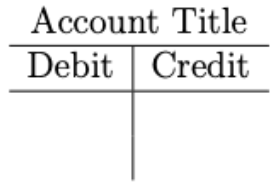
\includegraphics[scale=0.5]{t-account}
\begin{itemize}
	\item Every transaction there will be equal amounts listed
	\item Debit: Asset increase (eg. Withdrawals, Expenses)
	\item Credit: Liability, equity increase (eg. Revenue)
\end{itemize}
\begin{description}
	\item Permanent vs temporary accounts
	\item[Temporary]{Track accounts only during current period}
	\item[Permanent]{Capital accounts that track equity long-term}
	\item[Trade debtors]{Customer that has not paid for goods and services}
	\item[Trade creditor]{Supplier who has sent your business goods/services but haven't paid}
\end{description}
\keyword{Journal entries}{Convenient format for recording transactions}
%-----------------------------------------------------------------------------------------------------------------------
\section{05. Adjusting and closing}
\subsection{Adjusting entries}
Record of transactions happening during period that were unrecorded (Why unrecorded)
\begin{enumerate}
	\item Frequent or continuous transactions - impractical to record 
	\item Earning revenue/incurring expenses do not happen during cash payments (Prepayments/ accrued revenues and expenses)
	\item \keyword{Depreciation}{Adjustment for age of a long-lived asset used in business}
	\begin{tabbing}
		\= \keyword{Accumulated Depreciation}{Contra asset storing negative adjustment}
		\\\= Goes up on credit side and down on debit side\\
		\= \keyword{Carrying value}{Remaining value of asset (cost - accumulated depreciation)}
	\end{tabbing}
\end{enumerate}

\subsection{Closing entries}
Clear the temporary accounts
\\Capital(post-closing) = Capital(pre-closing) + Revenues - Expenses - Withdrawals
\subsubsection{Steps}
\begin{enumerate}
	\item Close revenue accounts to income summary (Debit revenue, credit income summary)
	\item Close expense accounts to income summary (Credit expense, debit income summary)
	\item Close income summary to capital
	\begin{itemize}
		\item Debit $>$ Credit: Debit balance $\rightarrow$ Net loss (Credit income summary balance, debit capital)
		\item Credit $>$ Debit: Credit balance $\rightarrow$ Net profit (Debit income summary balance, credit capital)
	\end{itemize}
	\item Close withdrawals account directly to Capital (Credit withdrawals, debit capital)
\end{enumerate}
%-----------------------------------------------------------------------------------------------------------------------
\section{06. Inventory}
\subsection{Sales and cost of goods sold}
\subsubsection{Transactions}
\begin{enumerate}
	\item Earned revenue (Sales revenue and cash/accounts receievable increase)
	\item Goods sold (Inventory and COGS expense decrease)
\end{enumerate}
\subsubsection{Perpetual System}
\begin{itemize}
	\item Tracks on every sale 
	\item vs \keyword{Periodic}{Compare beginning + purchases and ending inventory}
\end{itemize}
\subsection{Shrinkage}
Inventory is less than beginning (Unaccounted damage, loss)
\subsubsection{Min(Cost, NRV)}
\keyword{Cost}{Cost to acquire and make inventory available for sale}
\begin{itemize}
	\item Purchase price, NET of discounts or allowance
	\item Shipping cost (\keyword{Freight-in}{borne by the buyer})
	\item Taxes on purchase transaction (as long as not recoverable)
\end{itemize}
\keyword{Net Realizable Value}{Value that inventory can be sold, net reasonable cost to sell}
\subsection{Cash flow assumption}
\begin{itemize}
	\item \keyword{Specific identification}{Unique items that have to be tracked and use actual original cost of item}
	\item \keyword{Interchangeable goods}{Indistinguishable goods, typically in bulk}
	\begin{enumerate}
		\item FIFO
		\item Weighted average cost - Cost of each good are the same at the time of sale
	\end{enumerate}
\end{itemize}


%-----------------------------------------------------------------------------------------------------------------------

\section{Midterm}
Debits
\begin{description}
	\item[Assets]{Cash, Account receivables. Supplies/inventory, \textbf{PREPAID} insurance/rent, equipment, land, buildings}
	\item[Decrease in equity]{withdrawals, expenses(cost of goods sold)}
\end{description}
Credits
\begin{description}
	\item[Increase in equity]{Capital, revenue}
	\item[Increase in liabilities]{Accounts payable, accumulated depreciation, borrowing}
\end{description}

\section{07. Cash and A/R}
\begin{itemize}
	\item Cash at hand
	\item Cash in bank
	\item Cash equivalents (liquid, in safe financial instruments)
\end{itemize}
\subsection{Petty cash}
\begin{itemize}
	\item Fixed amount that companies holds, usually to meet day-to-day spending needs
	\item Credit "cash at bank" and debit "petty cash account" only when fund amount changes OR during setup/tear down
\end{itemize}
\subsubsection{Cash over and short}
\begin{itemize}
	\item Account representing the gap between expected amount from receipts and actual amount in petty cash box
	\item Accidental mistakes eg. petty cashier returning the wrong amount of change	
	\item Debited as minor expense
\end{itemize}
\subsubsection{Changing fund amount}
\begin{itemize}
	\item Record replenishment and amount to increase[debit]/decrease[credit] fund to petty cash
\end{itemize}
\subsection{Bank reconciliation}
\begin{itemize}
	\item Updating cash at bank records and book records (deposits and withdrawals)
\end{itemize}
\subsubsection{Causes}
\begin{description}
	\item[Deposits in transit]{Company received and recorded cheques and deposited in bank but bank has not cleared/recorded deposit \textbf{add to bank}}
	\item[Outstanding cheques]{Payment made via cheques but payee has not deposited cheques/still being processed}
	\begin{itemize}
		\item Bank has not deducted from account but book records payments when cheques were sent - \textbf{subtract from bank}
	\end{itemize}
	\item[Non-sufficient funds(NSF)]{Receive cheques that recorded as cash receipt and deposited but bounced because not enough money in payer bank account}
	\begin{itemize}
		\item Book incorrectly add amount \textbf{subtract from book}
	\end{itemize}
	\item[Bank charges]{Expense from commission fees and penalties deducted from account - \textbf{subtract from books}}
	\item[Interest received]{Commercial bank giving interest to account \textbf{add to book}}
	\item[Collections on behalf]{Bank directly collect outstanding dues on behalf \textbf{add to book}}
\end{description}
\subsection{Bad debts}
Accrual accounting at the end of the year
\begin{itemize}
	\item Expected loss from customers not paying when selling goods on credit
	\item Recorded as \textit{loss allowance} or \textit{allowance for bad debts}
	\item Contra-asset representing a negative adjustment to trade receivables
	\item Goes up on credit side and down on debit side
	\item Coupled with \textit{expected credit loss} or \textit{bad debt expense}
\end{itemize}
When customer defaults
\begin{itemize}
	\item Reduce allowance to "write off" trade receivable amount
	\item Can reverse write off (customer pays up despite giving up hope)
	\begin{itemize}
		\item Credit allowance and debit trade receivables
	\end{itemize}
\end{itemize}
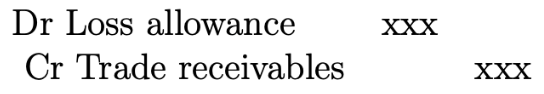
\includegraphics[scale=0.4]{write-off}
\section{08. Notes and Warranty}
\begin{itemize}
	\item Current liability
	\begin{itemize}
		\item Notes payable
		\item Warranty liability
	\end{itemize}
\end{itemize}
\subsection{Notes payable/receivable}
\begin{itemize}
	\item Formal document where a borrower promises to pay a fixed sum of money (principal) after a fixed period from date note is signed (issue date)
	\item Current asset (less than a year)
	\item Stronger than accounts payable/receivables
	\item \keyword{Maturity/settlement date}{Note due date}
	\item \keyword{Interest}{Additional amount borrower must return on top of principal (accrued interest + principal lumpsum)}
	\item Note that interest is recorded in a separate account with adjusting journal entries
\end{itemize}
\subsubsection{Calculations}
\begin{itemize}
	\item Months
	\begin{itemize}
		\item Taken from the same day of the month
		\item eg. Borrowing on 2/1/2023 + 3 months = 2/4/2023
	\end{itemize}
	\item Days
	\begin{itemize}
		\item Taken from the day after issue date
		\item eg. Borrow on 2/1/2023 + 30 days = 1/2/2023
	\end{itemize}
	\item Record non-payments against an established allowance
\end{itemize}
\subsubsection{Provisions liabilities}
\begin{itemize}
	\item Liabilities where timing and amount are uncertain and needs to be estimated
	\item eg. \keyword{embedded warranty}{Warranty automatically gotten when purchasing goods(included in sale price)}
	\item vs \keyword{extended warranty}{Extra charge for additional warranty counted under unearned revenue}
	\item \keyword{Warranty expense}{Balancing figure when creating/increasing provision}
	\item \keyword{Warranty liability}{Anticipated future claims decrease when actual warranty claim occurs (cash/asset goes down concurrently)}
\end{itemize}
\subsubsection{Contingent liabilities}
\begin{itemize}
	\item Possible uncertain liabilities that do not satisfy the criteria to be stated as provisions
\end{itemize}

\section{09.PPE}
\begin{itemize}
	\item Tangible long-lived assets used in business to generate profits
	\item Life is more than a year (non-current asset)
\end{itemize}
\subsection{Accounting}
\begin{itemize}
	\item Initially recorded at acquisition cost
\end{itemize}
\begin{enumerate}
	\item Cost approach
	\begin{itemize}
		\item Asset recorded at \keyword{carrying amount}{cost less accumulated depreciation}
		\item Recorded by 2 accounts (PPE at cost and accumulated depreciation on PPE)
	\end{itemize}
	\item Revaluation approach
	\begin{itemize}
		\item Periodically revalued to current market value
		\item Record the difference in value as accumulated depreciation
	\end{itemize}
\end{enumerate}
\subsection{Acquisition cost}
\begin{itemize}
	\item Includes all cost necessary to acquire asset, bring to location of use and install it
	\item Additional cost accrued as initial acquisition cost of asset
	\item Includes future cost of dismantling/clean-up of assets
	\item All related liability is non-current
	\item If bought as a bundle
	\begin{enumerate}
		\item Sum standalone price for each item in bundle
		\item Get ratio of standalone item price to sum
		\item Bundle price * ratio = acquisition cost of item
	\end{enumerate}
\end{itemize}

\subsection{Capital vs Revenue expenditure}
Cost incurred after installation
\subsubsection{Capital expenditure}
\begin{itemize}
	\item Addition or improvement of assets
	\item Provides additional functionality and extends life
	\item Increase in asset at cost amount
\end{itemize}
\subsubsection{Revenue expenditure}
\begin{itemize}
	\item Routine repair, maintenance/cleaning cost to maintain in proper working conditions
	\item Recorded as expense
\end{itemize}

\subsection{Depreciation}
\begin{itemize}
	\item Estimate of the wear and tear that assets suffers during life
\end{itemize}
\subsubsection{Straight-line depreciation}
$\dfrac{Acquisition~cost-Residual~value~if~any}{life~in~years}$
\subsubsection{Partial-year depreciation}
\begin{itemize}
	\item Acquired during a year so depreciation is prorated at a fraction of a year (rounded to nearest month)
	\item \keyword{15-day rule}{Before 15 start counting from that month, after 15th start counting from next month}
\end{itemize}
\subsubsection{Revising assumptions}
Estimate of depreciation changes
\begin{itemize}
	\item Revised estimates \textbf{prospectively} over the remaining recalculated life of asset
	\item Not \keyword{retrospectively}{Changing past estimates}
	\item Revised depreciation expense =
	\item $\dfrac{carrying~amount~at~beginning~of~year-Revised~residual~value}{Revised~remaining~life~from~start~of~year}$
\end{itemize}

\subsection{PPE disposal}
\subsubsection{Selling PPE}
Steps:
\begin{enumerate}
	\item Credit PPE asset \textbf{at cost} to 0
	\item Debit accumulated depreciation of PPE asset to make it 0
	\item Debit proceeds from sale to cash/receivable
	\item Gain [Credit] or loss[debit] on disposal
	\begin{itemize}
		\item Proceeds from sale of PPE - carrying amount of PPE at sale date
	\end{itemize}
\end{enumerate}

\section{10. Corporations}
\begin{itemize}
	\item Ownership is divided into a number of shares of the net worth - entitles holder to ownership of a fraction of the company
	\item \keyword{Share capital}{Value of the investment made in the company by share investors when shares are issued by company}
	\item \keyword{Retained earnings}{Value of accumulated net profits earned by the company so far in life (less accumulated dividents paid/commited to pay}
	\item Equity - original investment made by shareholders when shares are issued + amount added to net worth by accumulated net profit that has not been paid back
\end{itemize}
\subsection{Cash dividends}
Important dates
\begin{description}
	\item[Declaration date]{Date company records the dividend (as direct debit to retained earnings)}
	\item[Date of record]{Cutoff date for the recipient of the dividend (no entry on the day)}
	\item[Payment date]{Date where the dividend is paid}	
\end{description}

\subsection{Other Comprehensive Income}
\begin{itemize}
	\item Represents movements in equity not recorded in income statement since they are remeasurement of assets/liabilities rather than actual income/expenses
	\item Recorded separately from net profit which sums to form `Comprehensive Income`
	\item Accumulated in a permanent equity account (reserve) and contra-asset (accumulated OCI of the particular type)
	\item eg. Property revaluation, retained earnings
\end{itemize}

\subsection{Preference Shares}
\begin{itemize}
	\item No voting rights
	\item Pay fixed dividends calculated using standard dividend rate per annum based on fixed nominal value per share
	\item Dividends are non compulsory, but rank higher than ordinary shares (company have to pay preference before ordinary dividends)
	\item May be :
	\begin{description}
		\item[Cumulative]{Includes value from last year}
		\item[Convertible]{Can be converted to ordinary shares}
		\item[Redeemable]{Company promises to buy them back at a fixed price}
	\end{description}
\end{itemize}

\subsection{Treasury Shares}
\begin{itemize}
	\item Shares bought back by company but not cancelled (held in treasury)
	\item Cannot vote or receive dividends but can be reissued
	\item Recorded as a negative adjustment to equity inside the equity section (contra-equity account, debit)
	\item Recorded at cost - Price paid by company when bought back
\end{itemize}

\subsection{Bonus Shares}
\begin{itemize}
	\item Free shares given to existing shareholders (purely cosmetic)
	\item There is usually no entry to record bonus issue
	\item However, can be used to transfer some amount from retained earnings to share capital
	\begin{itemize}
		\item To meet legal or contractual requirements
		\item Bonus issues stated to be at some notional issue price
	\end{itemize}
\end{itemize}

\section{11. Statement of Cash Flows (SCF)}
\begin{itemize}
	\item Used to determine cash flows analytically by deriving from accrual-basis financial statements
	\item Cash + other assets = Liabilities + equity
	\item Interest received and dividends paid could be operating/financing section
	\item Net change in cash/cash equivalents (sum of cash flows in 3 sections) = difference between opening and closing balance in balance sheet
	\item Combined with other liquid short-term assets called cash equivalents like fixed D or overdraft
\end{itemize}
\subsubsection{Operating Activities}
\begin{itemize}
	\item Business operations of the enterprise 
	\item Reflect most changes in retained earnings, non-cashg current assets arising from operations and current liabilities
\end{itemize}

\subsubsection{Investing Activities}
\begin{itemize}
	\item From investing or divesting in non-current assets company uses for business/side-investment
	\item Records changes in non-current assets, cash in/outflow from acquiring investment shld be shown separately not netted (from sale of investment)
	\item Significant non-cash transactions shld be disclosed separately in notes
\end{itemize}

\subsubsection{Financing Activities}
\begin{itemize}
	\item Transactions with suppliers of financing ie lenders and shareholders
	\item Derived from changes in borrowing (short/long term and changes in share capital)
	\item In/outflows should be recorded non netted like investing (same w non-cash transactions)
\end{itemize}

\subsection{Cash Flow From Operating activities (CFFO)}
Simplified algorithm to derive via indirect method:
\begin{itemize}
	\item[+] Profit before interest and tax
	\item[+] Non-cash expense item amounts (eg. depreciation expense)
	\item[-] Non cash income item amounts (eg. share on profits of associates)
	\item[$\pm$] Gain/loss on PPE disposal (investing section)
	\item[-] Change in operating current assets
	\item[+] Change in operating current liabilities
\end{itemize}

\subsubsection{Direct method}
\textbf{Cash collected from customers}
\begin{itemize}
	\item[+] Net Sales
	\item[-] Change in net trade receivables
	\item[+] Change in unearned sales revenue
	\item[-] Expected credit loss expense
\end{itemize}
\textbf{Cash paid to suppliers of merchandise}
\begin{enumerate}
	\item Estimate purchases of merchandise (Purchases = COGS + $\triangle$Inventory)
	\item Compute cash paid via change in trade payables (Cash paid = Purchases - $\triangle$Trade payables)
\end{enumerate}
\textbf{Income tax paid}
\begin{itemize}
	\item[+] Income tax expense
	\item[-] Change current income tax payable
	\item[-] Change deferred income tax liabilities
	\item[+] Change deferred income tax assets
\end{itemize}

\section{12. Financial Statement Analysis}
\subsection{Maunfacturing Companies}
\begin{itemize}
	\item Inventory accounting using "cost accounting"
	\item Types of inventory:
	\begin{itemize}
		\item Raw materials
		\item Work In Process/product item that are in process of being manufactured
		\item Finished goods ready for sale
	\end{itemize}
	\item Cost accumulated in WIP and finished goods must include material cost and other production cost (Conversion costs)
	\item Changes
	\begin{enumerate}
		\item Debit Raw materials when purchasing raw material and credit when using raw material (debit into WIP)
		\item WIP goes up by amount of raw materials used in production + conversion cost (goes down once completed)
		\item WIP go down = Finished goods go up as Cost of Goods Manufactured (COGM)
		\item When sold, finished goods go up on COGM and down on COGS 
	\end{enumerate}
\end{itemize}

\subsection{Bank accounting}
\begin{itemize}
	\item Bank is in the business of lending and borrowing cash so large proportion of interest charges are operating activities
	\item Only Interest paid on subordinate debt (tier 2) are financing, the rest should be operating section
\end{itemize}
\subsubsection{Return on Equity}
\begin{itemize}
	\item Contain preference shares so preference dividends must be calculated
	\item Calculation for group\\
	$\dfrac{Net~profit-NCI~share~profit-Pref~dividends}{AVG(Equi-NCI~share~equi-Pref~share~capital)}$
	\item Note: Denominator must not include accumulated unpaid preference share dividend from cumulative preference share
	\begin{itemize}
		\item Not considered part of the preference share portion of equity
	\end{itemize}
\end{itemize}

\subsubsection{Bank-specific ratios}
\begin{description}
	\item[Net interest margin (NMI)]{Spread between interest income earned and interest expense incurred as proportion of total assets}\\
	$\dfrac{Interest~income-Interest~expense}{Average~total~assets}$
	\item[Capital Adequacy ratio]{Regulatory ratio that banks have to maintain minimum of}
	\begin{description}
		\item[Common Equity Tier 1 (CET1)]
		$\dfrac{Common~equity~tier~1~capital}{Risk-weighted~assets}$
		\item[Tier 1 Capital Adequacy Ratio (CAR1)]
		$\dfrac{Tier~1~capital}{Risk-weighted~assets}$
		\item[Total Capital Adequacy ratio (Total CAR)]
		$\dfrac{Tier~1~Capital + Tier~2~Capital}{Risk-weighted~assets}$
	\end{description}
	\begin{itemize}
		\item Helps assess bank's ability to withstand bank run
		\item Protection that the depositors have against bank running out of funds and being unable to return deposits
		\item Dependent on the source of funds raised eg. Ordinary shares and accumulated reserves (Common Equity tier 1)
		\item Slightly less protective are instruments like Pref shares (Tier 1 Capital)
		\item Even lower are Low ranking subordinate debt (tier 2 capital)
		\item Compare with company assets (Loans or investments in financial instruments)
		\item Requires assessment of risks
		\begin{description}
			\item[Credit Risk]{Risk borrower will not repay what is owed}
			\item[Market Risk]{Risk that investment suffers decline in market value}
			\item[Operational Risk]{Asset used in operation suffers operational crisis (computer network being hacked)}
		\end{description}
	\end{itemize}
	\item[Non-Performing Loans (NPL)]{Loans on which payment is overdue by more than 90 days}\\
	$\dfrac{Non-performing~loans}{Gross~loans}$
\end{description}

\subsubsection{Financial Instruments}
\begin{itemize}
	\item Financial assets and liabilities 
	\begin{description}
		\item[Receivables]{Loans (assets), borrowings (liabilities), investment in shares or equity of other companies (assets)}
		\item[Derivatives]{Financial contracts that can be assets (+) or liabilities (-) depending on market value}
	\end{description}
\end{itemize}
\textbf{Financial asset classifications}
\begin{description}
	\item[Fair value through profit and loss (FVPL)]{Default category}
	\begin{itemize}
		\item Recorded at balance-sheet date market value (fair value)
		\item Changes in fair value recorded as gains or losses in income statement
	\end{itemize}
	\item[Fair value through OCI (FVOCI)]{Record loans/investment in shares at fair value whose changes recorded in OCI (rather than income statement)}
	\begin{itemize}
		\item Accumulated in separate reserves called FVOCI revaluation reserve
	\end{itemize}
	\item[Amortized cost]{Used for financial liabilities mostly (except derivatives - recorded at FVPL)}
	\begin{itemize}
		\item Loans held to maturity and never sold
		\item Company recorded at cost less repayments and plus accrued interest
	\end{itemize}
\end{description}
\section{Finals prep}
\subsection{Costs}
\begin{description}
	\item[COGM]{Cost of goods manufactured = COGS + $\triangle$final goods}
	\item[Cost of production]{COGM + $\triangle$unfinished goods}
\end{description}
\subsection{Impairments}
\begin{itemize}
	\item Permanent reduction in value of company asset
	\item Asset's fair value is less than its carrying value on the balance sheet
	\item Impairment only detected during testing as an impairment loss
\end{itemize}
\subsection{Chow Sang}
\subsubsection{PPE (15.140-142)}
\begin{itemize}
	\item Buildings were revalued so impairment loss due to new valuation
	\item Original carry amount = 6,873,000
\end{itemize}
\subsubsection{Credit loss for account receivables (22.151)}
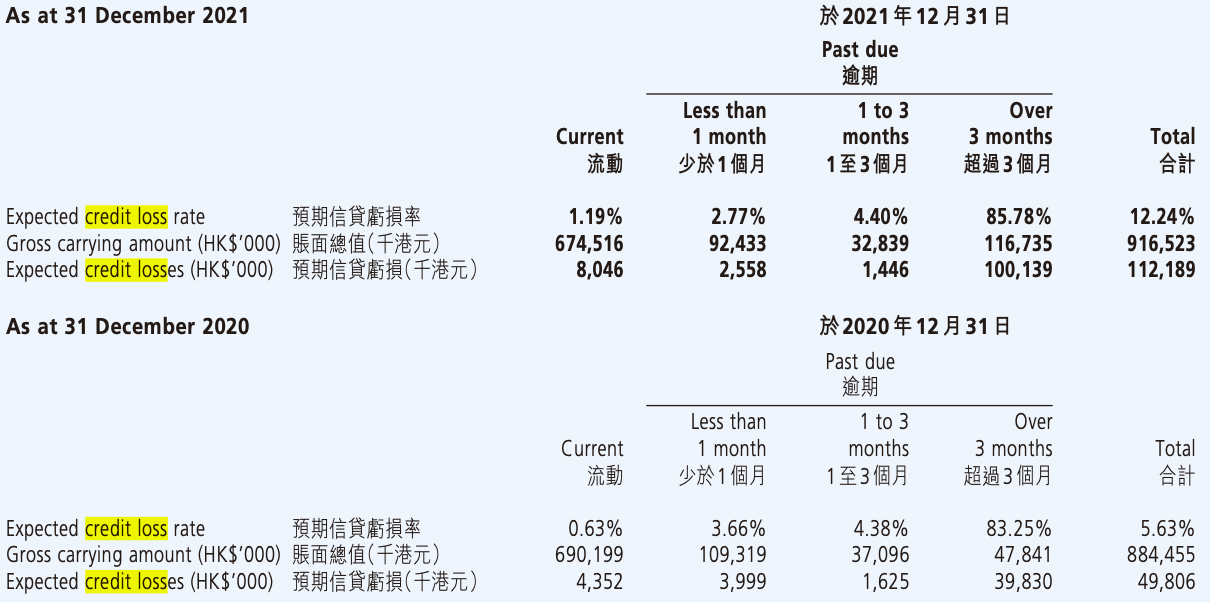
\includegraphics[scale=0.4]{acc-receivable-credit-loss}
\subsubsection{Share option schemes (35.167)}
\begin{itemize}
	\item Old scheme - Employees get shares that can be exercised at 14.89
	\item New scheme - Exercise price is highest of 
	\begin{itemize}
		\item Closing price of shares stated in stock exchange
		\item Average closing price for 5 busi days
		\item Nominal value of share
	\end{itemize}
\end{itemize}
\subsection{Debit credit}
\begin{description}
	\item[Debit]{Trade debtors, cash, inventory, expenses, Cost of goods sold, PPE at cost, Withdrawals, Receivables, Prepaid expense}
	\item[Credit]{Revenue, Accumulated depreciation, Share capital, Loss allowance on debtors, impairments, borrowings, creditors, retained earnings, Payables, Unearned revenue}
\end{description}
\end{multicols*}
\end{document}
